The hadronic decay of $\tau$ leptons (\tauh) is one of the largest components of the background from \ttbar , $W$+jets and single-top events contributing to the search regions. Isolated tracks veto is applied in the baseline selection to reduce the hadronic $\tau$ background while sustaining a minimal impact on signal efficiency. After applying the veto, the remnant hadronic $\tau$ events are estimated using the method described as following.

When a $W$ boson decays to a neutrino and a hadronically decaying $\tau$ lepton ($\tauh$), the presence of neutrinos in the final state results in \MET, and the event passes the lepton veto because the hadronically decaying $\tau$ is reconstructed as jets. This background is estimated from a control sample (CS) of $\mu$\,+\,jets 
events selected from data using a $\mu+\HT$-based trigger, 
HLT\_Mu15\_IsoVVVL\_PFHT350\_v, and requiring exactly one 
$\mu$ with $p_{T}^{\mu}>20 GeV$ and $|\eta|<2.4$.
A cut on the transverse mass of the $W$, 
$m_\mathrm{T}=\sqrt{2p_{T}^{\mu}\MET(1-\cos\Delta\phi)}<$ 100 GeV, 
is required in order 
to select events containing a $W\to\mu\nu$ decay and to suppress 
possible new physics signal contamination, i.e., signal events
present in the $\mu$\,+\,jets sample. Here,
$\Delta\phi$ is the azimuthal angle between the $\vec{p_{T}}^\mu$ and the 
\MET directions.
Because the $\mu$\,+\,jets and \tauh{}\,+\,jets events arise from the same 
physics processes, the hadronic component of the two samples is the same 
except for the response of the detector to the muon or the $\tauh$ jet. 
The trick consists of replacing the muon $p_{T}$ by a random sample of a
simulated \tauh jet response "template" function for a 
hadronically-decaying $\tau$ lepton. The 
global variables of the event are recalculated with this $\tauh$ jet, and the 
search selections are applied to predict the \tauh background.

As shown in Fig.~\ref{fig:templates}, the template is measured in four $p_{T}$ bins to account for the $p_{T}$ dependence of $\tau$ jet response.

\begin{figure}[htbp]
\centering
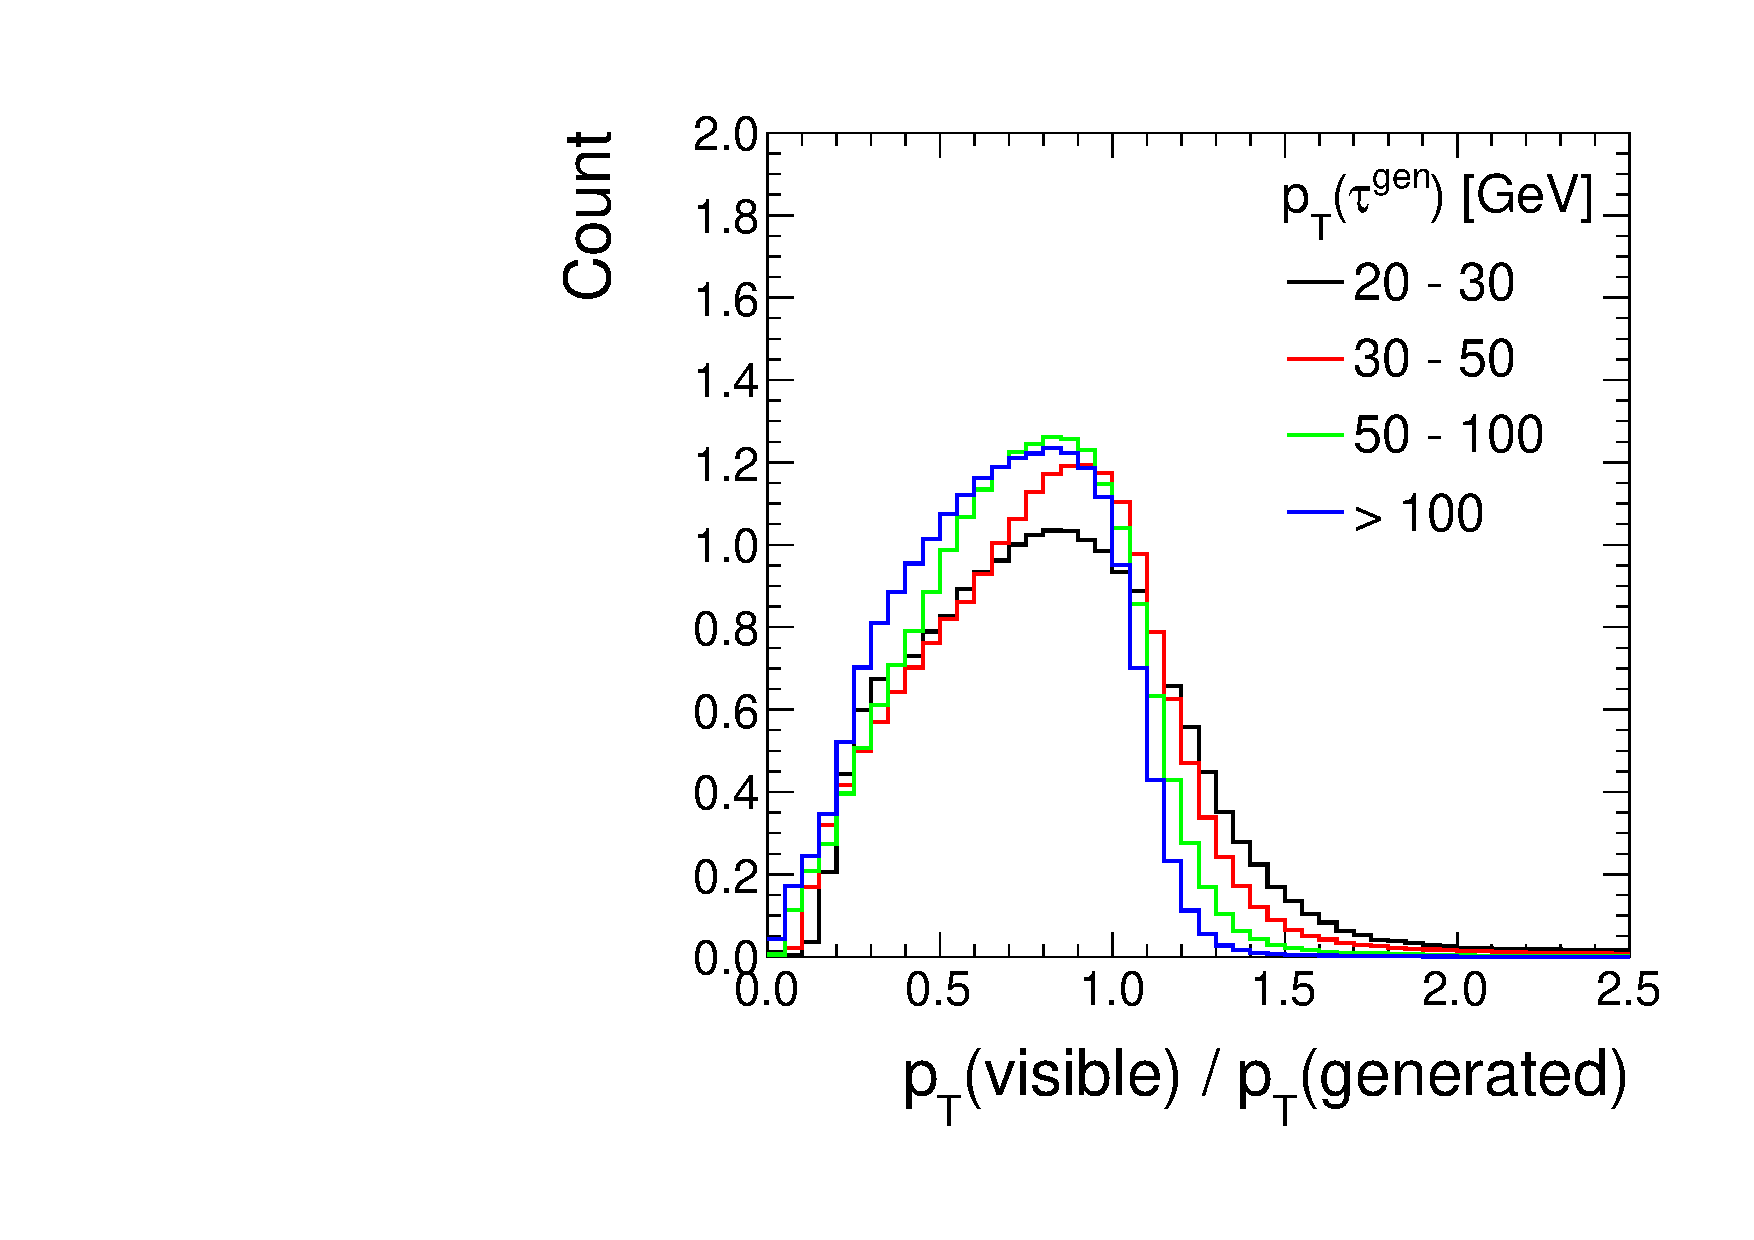
\includegraphics[width=0.5\textwidth]{sections/mc4/Backgrounds/HadTau/figures/TauResponseTemplate.pdf}
\caption{Tau jet visible energy fraction templates in tau lepton $p_{T}$ bins.}
\label{fig:templates}
\end{figure}

The $\tauh$ background prediction is calculated as follows:
\begin{equation}
N_{\tau_{h}} = \sum\limits_i^{N_\mathrm{CS}^\mu}\left(\sum\limits_j^\text{Template bins}(P_{\tau_h}^\text{resp})
\frac{\epsilon_{\tau \rightarrow \mu}}{\epsilon^{\mu}_\text{trigger}\,\epsilon^{\mu}_\text{reco}\,\epsilon^{\mu}_\text{iso}\,\epsilon^{\mu}_\text{acc}\,\epsilon^{\mu}_{m_\text{T}}} \dfrac{ \mathcal{B}(W \rightarrow \tau_h)}{\mathcal{B}(W \rightarrow \mu)}\,\epsilon_\text{isotrack}\,F_\text{dilepton}\right)
\label{eq:tauh}
\end{equation}
where the first summation is over the events in the $\mu$ + jets control sample, the second is over the bins of the $\tau_h$ response template and $P_{\tau_h}^{resp}$ is the probability of $\tau_h$ response from each bin.

The classical hadronic tau method is not applied in this analysis because of the issue in the HT bit L1 trigger in 2016 run H data.
